\section{Introduction}
\begin{frame}{\VideoName}
    \tableofcontents[currentsection]
\end{frame}

\begin{frame}{Confusion and diffusion}
    \begin{itemize}
        \item For the construction of symmetric block ciphers, two important principles are followed by modern cryptographers -- \textit{confusion} and \textit{diffusion}.
        \item Shannon first introduced them in his famous paper\footnote{Claude E Shannon. A mathematical theory of cryptography. Mathematical Theory of Cryptography, 1945}
        \item Confusion obscures the relationship between the ciphertext and the key.
        To achieve this, each part of the ciphertext should depend on several parts of the key.
       \item Diffusion obscures the statistical relationship between the plaintext and the ciphertext.
       Each change in the plaintext is spread over the ciphertext, with the redundancies being dissipated.
       % \begin{itemize}
       %      \item For example, affine cipher has very low diffusion -- the distributions of letters in plaintext correspond directly to those in the ciphertext.
       %      \item That is also why frequency analysis can be applied to break those ciphers.
       % \end{itemize}
    \end{itemize}
\end{frame}

\begin{frame}{Block cipher design specifications}
    \begin{itemize}
        \item A symmetric block cipher design specifies a \textit{round function} and a \textit{key schedule}.
        \item Encryption of a plaintext block consists of a few \textit{rounds} of round functions, possibly with minor differences.
       \item Each round function takes the cipher's current \textit{state} as an input and outputs the next state.
       \item The key schedule takes the master key $k$ and outputs the keys for each round, which are called \textit{round keys}.
       \item In most cases, the key schedule is an invertible function.
       \begin{itemize}
           \item Given one or more round keys, the master keys can be calculated.
       \end{itemize}
    \end{itemize}
\end{frame}

\begin{frame}{Physical attacks}
    \begin{itemize}
        \item By Kerckhoffs' principle
        \begin{itemize}
            \item round functions and key schedule specifications are public
            \item master key (hence also the round keys) are secret
        \end{itemize}
        \item We will only consider ciphers whose key schedules are invertible functions
        \item In physical attacks that we will discuss in the later parts of the book, the attacker normally aims to recover some round key(s) and then use the inverse key schedule to find the master key.
    \end{itemize}
\end{frame}

\begin{frame}{Encryption of a block cipher}
    \begin{itemize}
        \item $F$: round function  
        \item \texttt{Nr}: total number of rounds
        \item $K_i$: round key for round $i$
        \item $S_i$: the cipher state at the end of round $i$
        \item For a plaintext $p\in\FF_2^n$, the ciphertext $c\in\FF_2^n$ can be computed as follows\footnote{The round function for the last round might be a bit different, as for the case of AES}
    \end{itemize}
    \begin{eqnarray*}
    S_0 &=& p,\\
    S_1 &=& F(S_0,K_1),\\
    S_2 &=& F(S_1,K_2),\\
    &\vdots&\\
    S_{\texttt{Nr}} &=& F(S_{\texttt{Nr}-1},K_{\texttt{Nr}}),\\
    c &=& S_{\texttt{Nr}}.
    \vspace*{-0.5cm}
\end{eqnarray*}
\end{frame}

\begin{frame}{Decryption of a block cipher}
    \begin{itemize}
        \item To perform decryption, we require that for any given round key $K_i$, $F(\boldsymbol{x}, K_i)$ has an inverse, i.e.
\[
F^{-1}(F(\boldsymbol{x},K_i),K_i)=\boldsymbol{x},\quad \forall \boldsymbol{x}\in\FF_2^n.
\]
\item In this case, given ciphertext $c$, plaintext $p$ can be computed as follows:
\end{itemize}
\begin{eqnarray*}
S_{\texttt{Nr}} &=& c,\\
S_{\texttt{Nr-1}} &=& F^{-1}(S_{\texttt{Nr}},K_{\texttt{Nr}}),\\
&\vdots&\\
S_1 &=& F^{-1}(S_2,K_2),\\
S_0 &=& F^{-1}(S_1,K_1),\\
p &=& S_0.
\end{eqnarray*}
\end{frame}

\begin{frame}{\texttt{XOR} with the round key}
    \begin{itemize}
        % \item We recall for a vector space over $\FF_2$, vector addition is given by bitwise \texttt{XOR}, denoted $\oplus$ 
        \item \texttt{XOR} with the round key is a common operation in round functions of symmetric block ciphers.
    \end{itemize}
    \begin{example}
Take $111,101\in\FF_2^3$, 
\[
111\oplus 101=010
\]
    \end{example}
\end{frame}

\begin{frame}{Sbox}
    \begin{itemize}
        \item Another common function is a substitution function called \textit{Sbox}, denoted SB
        \item SB$:\FF_2^{\omega_1}\to\FF_2^{\omega_2}$.
        \item Normally $\omega_1$ or/and $\omega_2$ is a divisor of the block length $n$ and a few Sboxes are applied in one round function.
        \item When $\omega_1=\omega_2$, SB is a permutation on $\FF_2^{\omega_1}$ and we say that the Sbox is a \textit{$\omega_1-$bit Sbox}.
    \end{itemize}
\end{frame}

\begin{frame}{Feistel cipher and SPN cipher}
\begin{itemize}
    \item There are mainly two types of symmetric block ciphers -- \textit{Feistel cipher} and \textit{Substitution–permutation network (SPN) cipher}.
    \item Feistel: DES
    \item SPN: AES, PRESENT
\end{itemize} 
\end{frame}

\section{DES}
\begin{frame}{\VideoName}
    \tableofcontents[currentsection]
\end{frame}

\begin{frame}{Feistel cipher}
    \begin{itemize}
        \item The cipher state at the beginning/end of each round is divided into two halves of equal length.
        \item The cipher state at the end of round $i$ is denoted as $L_i$ and $R_i$, $L$ -- left, $R$ -- right.
        \item The round function $F$ is defined as 
\begin{equation*}
    (L_i, R_i)=F(L_{i-1},R_{i-1}, K_i), \text{ where } L_i=R_{i-1},\  R_i=L_{i-1}\oplus f(R_{i-1}, K_i).
\end{equation*}
\item We note that $f$ is a function that does not need to have an inverse since the function $F$ is always invertible
\[
L_{i-1}=R_i\oplus f(L_i,K_i),\quad R_{i-1}=L_i.
\]
\item The ciphertext is normally given by $R_{\texttt{Nr}}||L_{\texttt{Nr}}$ (i.e. swapping the left and right side of the cipher state at the end of the last round).
\item In this case, if we let $R_i$ and $L_i$ denote the right and left part of the cipher state at the end of round $i$ in the decryption, then the decryption computation is the same as for encryption, with round keys in reverse order
    \end{itemize}
\end{frame}

\begin{frame}{Feistel cipher}
    \begin{figure}[htb]
    \centering
    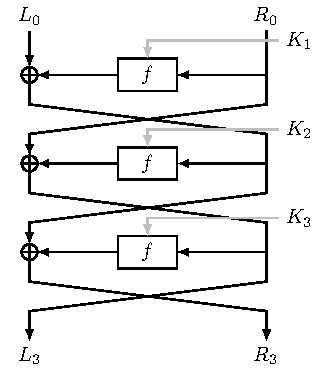
\includegraphics[width=0.45\textwidth]{fig/Feistel_Cipher.pdf}
    \caption{An illustration of Feistel cipher encryption algorithm.}
\end{figure}
\end{frame}

\begin{frame}{Data Encryption Standard (DES)}
    \begin{itemize}
        \item Developed at IBM by a team led by Horst Feistel and the design was based on Lucifer cipher.
        \item It was used as the NIST standard from 1977 to 2005.
        \item Even though the key length is too small for the current standard, some variants are still in use today
        \item It has a significant influence on the development of cipher design.
    \end{itemize}
\end{frame}

\begin{frame}{DES}
    \begin{itemize}
        \item The block length of DES is $n=64$, i.e. $\mathcal{P}=\mathcal{C}=\FF_2^{64}$.
        \item $L_i,R_i\in\FF_2^{32}$.
        \item The master key length is $56$, i.e. $\mathcal{K}=\FF_2^{56}$.
        \item The round key length is $48$.
        \item The total number of rounds $\texttt{Nr}=16$.
    \end{itemize}
    \begin{tikzpicture}[remember picture,overlay]
    \node[xshift=-4.5cm,yshift=2.5cm] at (current page.south east) {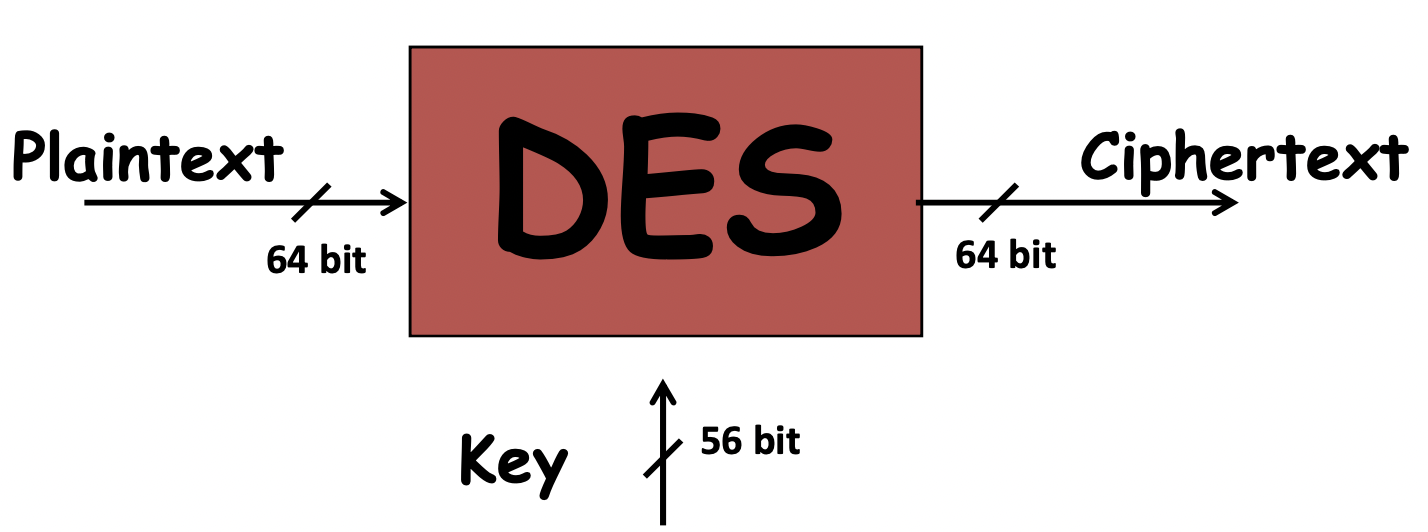
\includegraphics[width = 0.6\textwidth]{fig/DES.png}};
    \node[xshift=-4cm,yshift=0.3cm] at (current page.south east)
    {\picsrc{https://www.lri.fr/~fmartignon/}};
\end{tikzpicture}
\end{frame}

\begin{frame}{}
    \begin{figure}[htb]
    \centering
    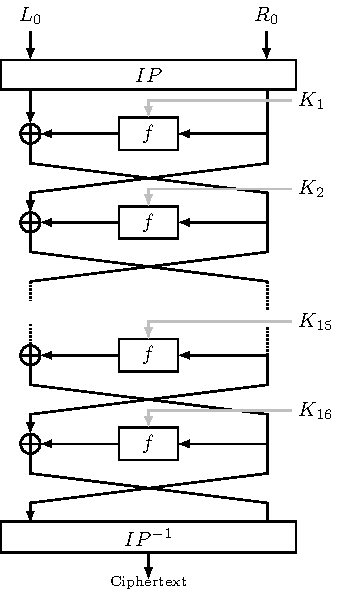
\includegraphics[width=0.35\textwidth]{fig/DES.pdf}
    % \caption{An illustration of DES encryption algorithm.}
\end{figure}
\end{frame}

\begin{frame}{DES -- function $f$}
    \begin{itemize}
        \item At the $i$th round, the function $f$ in the round function of DES takes input $R_{i-1}\in\FF_2^{32}$ and round key $K_i\in\FF_2^{48}$, then outputs a $32-$bit intermediate value:
\[
    f(R_{i-1},K_i)=P_{\text{DES}}(\text{Sboxes}(E_{\text{DES}}(R_{i-1})\oplus K_i)).
\]
    \end{itemize}
\begin{figure}
    \centering
    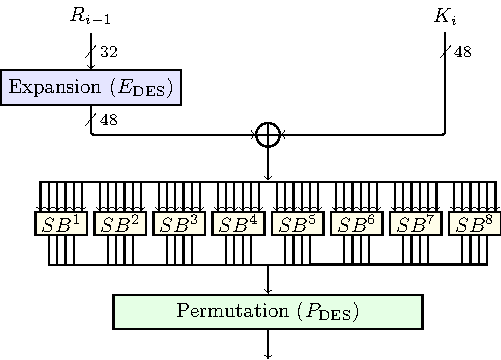
\includegraphics[width=0.6\textwidth]{fig/DES_F.pdf}
\end{figure}
\end{frame}

\begin{frame}{DES -- key schedule}
\begin{columns}[T] % align columns
\begin{column}{.6\textwidth}
\begin{itemize}
        \item Input: $64-$bit master key. Outputs round keys of length $48$.
        \item PC: \textit{permuted choice}
        \item Master key: each $8$th bit is a parity-check bit -- XOR of the previous $7$ bits
        \item PC1: $64$ bits are reduced to $56$ bits
        \item $56$ bits are divided into two $28-$bit halves
        \item Each half rotates left by one or two bits, depending on the round
        \item PC2: selects $48$ bits out of $56$ bits, permutes them
    \end{itemize}
\begin{alertblock}{Remark}
Knowledge of any round key $\to$ $48$ bits of the master key
\end{alertblock}
\end{column}%
\hfill%
\begin{column}{.5\textwidth}
\begin{figure}
    \centering
    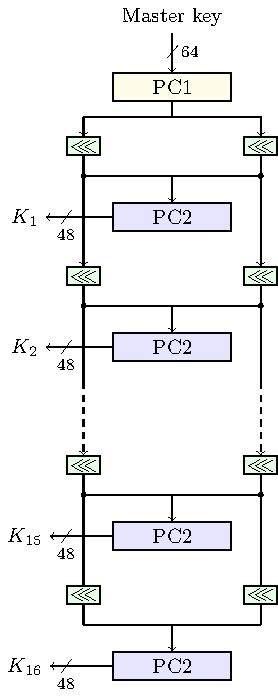
\includegraphics[width=0.7\textwidth]{fig/DES_KS.pdf}
\end{figure}
\end{column}%
\end{columns}
\end{frame}

\section{AES}
\begin{frame}{\VideoName}
    \tableofcontents[currentsection]
\end{frame}

\begin{frame}{SPN cipher}
    \begin{itemize}
        \item Let $\omega$ be a divisor of $n$, the block length, and let $\ell=n/\omega$.
        \begin{itemize}
            \item In most cases, $\omega=4,8$.
        \end{itemize}
       \item Each round of an SPN cipher normally consists of 
       \begin{itemize}
           \item bitwise \texttt{XOR} with the round key
           \item application of $\ell$ parallel $\omega-$bit Sboxes
           \item a permutation on $\FF_2^n$
       \end{itemize}
       \item The encryption starts with \texttt{XOR} with a round key, also ends with \texttt{XOR} with a round key before outputting the ciphertext, otherwise, the cipher states in the second (or the last) round are all known to the attacker.
       \begin{itemize}
           \item Those two operations are called \textit{whitening}.
       \end{itemize}
       \item For decryption, the inverse of Sbox and permutation are computed, and round keys are \texttt{XOR}-ed with the cipher state in reverse order compared to that for encryption.
    \end{itemize}
\end{frame}

\begin{frame}{}
    \begin{figure}[htb]
    \centering
    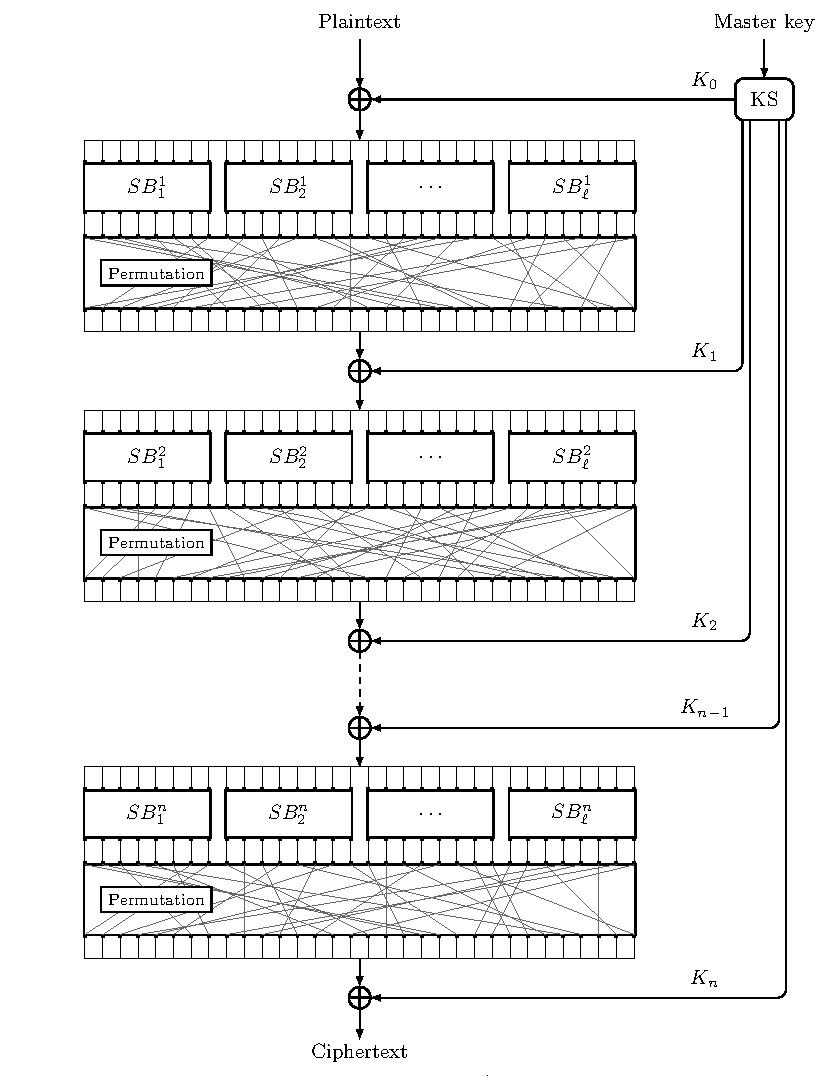
\includegraphics[width=0.48\textwidth]{fig/SPN_Cipher.pdf}
\end{figure}
\end{frame}

\begin{frame}{AES}
    \begin{itemize}
        \item NIST, 1997, Call for algorithms, replacement for DES
        \item Advanced Encryption Standard
        \item October 2000, Rijndael was selected
        \item Invented by Belgian cryptographers Joan Daemen and Vincent Rijmen
        \item Optimized for software efficiency on $8$ and $32$ bit processors
    \end{itemize}
\end{frame}

\begin{frame}{AES and Rijndael}
    \begin{itemize}
        \item $n=128$, $\omega=8$
        \item Number of rounds \texttt{Nr}$=10,12,14$
        \item Corresponding key length $=128,192,256$
        \item The original design of Rijndael also allows for different key lengths and block lengths.
    \end{itemize}
    \begin{table}[htb]
\centering
\begin{tabular}{|c|ccccc|}
\hline
\multirow{2}{*}{key length} & \multicolumn{5}{c|}{block length} \\ \cline{2-6} 
 & \textcolor{blue}{128} & 160 & 192 & 224 & 256 \\\hline
 \textcolor{blue}{128} & \textcolor{blue}{10} & 11 & 12 & 13 & 14\\
 160 & 11 & 11 & 12 & 13 & 14\\
 \textcolor{blue}{192} & \textcolor{blue}{12} & 12 & 12 & 13 & 14\\
 224 & 13 & 13 & 13 & 13 & 14\\
 \textcolor{blue}{256} & \textcolor{blue}{14} & 14 & 14 & 14 & 14\\\hline
\end{tabular}
\caption{Specifications of Rijndael design, where blue-colored values are adopted by AES.}
\end{table}
\end{frame}

\begin{frame}{AES encryption}
    \begin{itemize}
            \item An initial AddRoundKey
            \item Round function for \texttt{Nr}$-1$ rounds: SubBytes, ShiftRows, MixColumns, AddRoundKey
            \item Last round, round \texttt{Nr}: SubBytes, ShiftRows, AddRoundKey 
            \item AddRoundKey is bitwise \texttt{XOR} with the round key 
            \item SubBytes is the application of $8-$bit Sboxes.
             \item ShiftRows permutes the bytes 
             \item MixColumns is a function on $32-$bit values (four bytes).
        \end{itemize}
        \begin{figure}
        \centering
        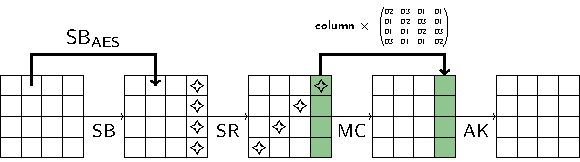
\includegraphics[width=0.9\textwidth]{fig/AES_round_function.pdf}
    \end{figure}
\end{frame}

\begin{frame}{AES -- decryption}
    \begin{itemize}
        \item The inverse of SubBytes, ShiftRows, and MixColumns are denoted as InvSubBytes, InvShiftRows, and InvMixColumns respectively.
        \item The first round of AES decryption computes AddRoundKey, InvShiftRows, and InvSubBytes.
        \item Then the round function for the next \texttt{Nr}$-1$ rounds consists of AddRoundKey, InvMixColumns, InvShiftRows, and InvSubBytes.
        \item Finally, an additional AddRoundKey is computed
        \item Round keys for decryption are in reverse order as those for encryption.
    \end{itemize}
\end{frame}

\begin{frame}{AES -- SubBytes}
\begin{table}[]
\ttfamily
\small
% \texttt
\begin{tabular}{c|cccccccccccccccc}
 & 0 & 1 & 2 & 3 & 4 & 5 & 6 & 7 & 8 & 9 & A & B & C & D & E & F \\\hline
0 & 63 & 7C & 77 & 7B & F2 & 6B & 6F & C5 & 30 & 01 & 67 & 2B & FE & D7 & AB & 76 \\
1 & CA & 82 & C9 & 7D & FA & 59 & 47 & F0 & AD & D4 & A2 & AF & 9C & A4 & 72 & C0 \\
2 & B7 & FD & 93 & 26 & 36 & 3F & F7 & CC & 34 & A5 & E5 & F1 & 71 & D8 & 31 & 15 \\
3 & 04 & C7 & 23 & C3 & 18 & 96 & 05 & 9A & 07 & 12 & 80 & E2 & EB & 27 & B2 & 75 \\
4 & 09 & 83 & 2C & 1A & 1B & 6E & 5A & A0 & 52 & 3B & D6 & B3 & 29 & E3 & 2F & 84 \\
5 & 53 & D1 & 00 & ED & 20 & FC & B1 & 5B & 6A & CB & BE & 39 & 4A & 4C & 58 & CF \\
6 & D0 & EF & AA & FB & 43 & 4D & 33 & 85 & 45 & F9 & 02 & 7F & 50 & 3C & 9F & A8 \\
7 & 51 & A3 & 40 & 8F & 92 & 9D & 38 & F5 & BC & B6 & DA & 21 & 10 & FF & F3 & D2 \\
8 & CD & 0C & 13 & EC & 5F & 97 & 44 & 17 & C4 & A7 & 7E & 3D & 64 & 5D & 19 & 73 \\
9 & 60 & 81 & 4F & DC & 22 & 2A & 90 & 88 & 46 & EE & B8 & 14 & DE & 5E & 0B & DB \\
A & E0 & 32 & 3A & 0A & 49 & 06 & 24 & 5C & C2 & D3 & AC & 62 & 91 & 95 & E4 & 79 \\
B & E7 & C8 & 37 & 6D & 8D & D5 & 4E & A9 & 6C & 56 & F4 & EA & 65 & 7A & AE & 08 \\
C & BA & 78 & 25 & 2E & 1C & A6 & B4 & C6 & E8 & DD & 74 & 1F & 4B & BD & 8B & 8A \\
D & 70 & 3E & B5 & 66 & 48 & 03 & F6 & 0E & 61 & 35 & 57 & B9 & 86 & C1 & 1D & 9E \\
E & E1 & F8 & 98 & 11 & 69 & D9 & 8E & 94 & 9B & 1E & 87 & E9 & CE & 55 & 28 & DF \\
F & 8C & A1 & 89 & 0D & BF & E6 & 42 & 68 & 41 & 99 & 2D & 0F & B0 & 54 & BB & 16
\end{tabular}
\end{table}
    SB$_{\text{AES}}(\texttt{12})=\texttt{C9}$
\end{frame}

\begin{frame}{AES -- MixColumns}
    \begin{itemize}
        \item Denote AES state
        \[
    \begin{pmatrix}
    s_{00} & s_{01} & s_{02} & s_{03}\\
    s_{10} & s_{11} & s_{12} & s_{13}\\
    s_{20} & s_{21} & s_{22} & s_{23}\\
    s_{30} & s_{31} & s_{32} & s_{33}
    \end{pmatrix}
    \]
    \item The MixColumns multiplies each column of the cipher state by a matrix:
\begin{equation}
    \begin{pmatrix}
    d_0\\
    d_1\\
    d_2\\
    d_3
    \end{pmatrix}
    =\begin{pmatrix}
    \texttt{02} & \texttt{03} & \texttt{01} & \texttt{01} \\
    \texttt{01} & \texttt{02} & \texttt{03} & \texttt{01} \\
    \texttt{01} & \texttt{01} & \texttt{02} & \texttt{03} \\
    \texttt{03} & \texttt{01} & \texttt{01} & \texttt{02}
    \end{pmatrix}
    \begin{pmatrix}
    s_{0j}\\
    s_{1j}\\
    s_{2j}\\
    s_{3j}
    \end{pmatrix},\quad j=0,1,2,3.
\end{equation}
\item Multiplication is done in a specific field
\begin{itemize}
    \item Multiplication by \texttt{01} does not change the value
    \item For any byte $b_7b_6\dots b_1b_0$, multiplication by \texttt{02} is equivalent to left shift by $1$ and \texttt{XOR} with $00011011=\texttt{1B}$ if $b_7=1$
    \item Multiplication by \texttt{03} is equivalent to first multiply by \texttt{02} then \texttt{XOR} with the byte itself
\end{itemize}
\item Addition is equivalent to XOR
    \end{itemize}
\end{frame}

\begin{frame}{AES-128 -- key schedule}
\begin{columns}[T] % align columns
\begin{column}{.65\textwidth}
\begin{itemize}
    \item The round keys are represented as four-by-four grids and each box corresponds to one byte
    \item The rotation $<<$ rotates the right-most column by one byte
\[
\begin{pmatrix}
    y_0\\
    y_1\\
    y_2\\
    y_3
\end{pmatrix}
\mapsto
\begin{pmatrix}
    y_1\\
    y_2\\
    y_3\\
    y_0
\end{pmatrix}.
\]
\item Round constants:
\[
\text{Rcon}=\Set{\texttt{01, 02, 04, 08, 10, 20, 40, 80, 1B, 36}}.
\]
\begin{alertblock}{Remark}
Knowledge of any round key of AES-128 $\to$ master key
\end{alertblock}
\end{itemize}
\end{column}%
\begin{column}{.68\textwidth}
\begin{figure}[htb]
    \centering
    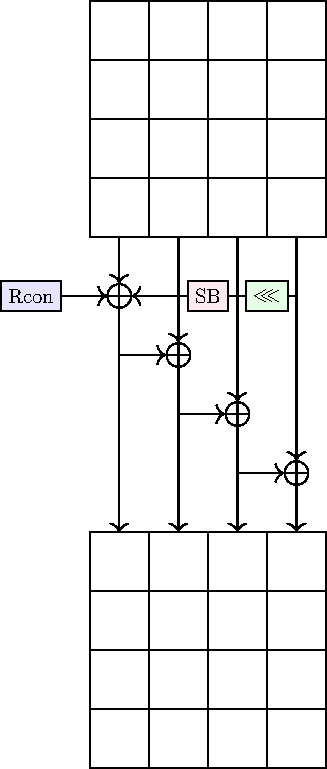
\includegraphics[width=0.34\textwidth]{fig/AES_KS.pdf}
\end{figure}
\end{column}%
\end{columns}
\end{frame}


\section{PRESENT}
\begin{frame}{\VideoName}
    \tableofcontents[currentsection]
\end{frame}

\begin{frame}{PRESENT}
    \begin{itemize}
        \item Proposed in 2007 as a symmetric block cipher optimized for hardware implementation.
       \item Block length: $n=64$
       \item Number of rounds: \texttt{Nr}$=31$
       \item Key length: either $80$ or $128$.
        \item When the key length is $80$, the algorithm is called PRESENT-80.
    \end{itemize}
\end{frame}

\begin{frame}{PRESENT -- encryption}
\begin{columns}[T] % align columns
\begin{column}{.55\textwidth}
\begin{itemize}
    \item Round function: addRoundKey, sBoxLayer, and pLayer.
    \item After $31$ rounds, addRoundKey is applied again before the ciphertext output 
\end{itemize}
\begin{alertblock}{Remark}
    For PRESENT specification, we consider the $0$th bit of a value as the rightmost bit in its binary representation.
For example, the $0$th bit of $3=011_2$ is $1$, the $1$st bit is $1$ and the $2$nd bit is $0$.
\end{alertblock}
\end{column}%
\hfill%
\begin{column}{.5\textwidth}
\begin{figure}
    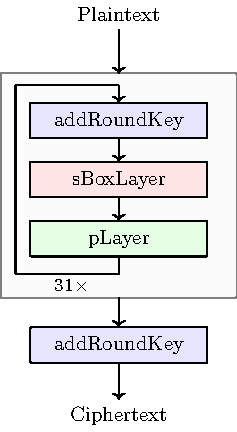
\includegraphics[width=0.55\textwidth]{fig/PRESENT.pdf}
\end{figure}
\end{column}%
\end{columns}
\end{frame}

\begin{frame}{PRESENT -- addRoundKey}
    \begin{itemize}
        \item Round key $K_i=\kappa^i_{63}\dots\kappa_0^i$, $(1\leq i\leq 32)$
        \item Current state $b_{63}b_{62}\dots b_0$
        \item For $0\leq j\leq 63$
    \end{itemize}
    \[
b_j= b_j\oplus\kappa_j^i
\]
\end{frame}

\begin{frame}{PRESENT -- sBoxLayer}
    \begin{itemize}
        \item sBoxLayer applies sixteen $4-$bit Sboxes to each nibble of the current cipher state.
        \item For example, if the input is \texttt{0}, the output is \texttt{C}.
\begin{table}[htb]
\centering
\ttfamily
\begin{tabular}{cccccccccccccccc}\hline
 0 & 1 & 2 & 3 & 4 & 5 & 6 & 7 & 8 & 9 & A & B & C & D & E & F \\\hline
 C & 5 & 6 & B & 9 & 0 & A & D & 3 & E & F & 8 & 4 & 7 & 1 & 2\\\hline
\end{tabular}
\end{table}
    \end{itemize}
\begin{figure}
    \centering
    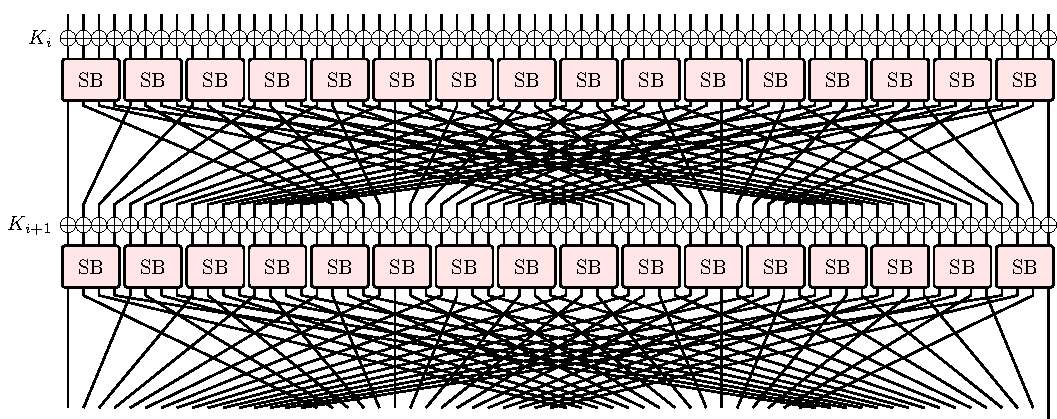
\includegraphics[width=0.9\textwidth]{fig/PRESENT_two_rounds.pdf}
\end{figure}
\end{frame}


\begin{frame}{PRESENT -- pLayer}
pLayer permutes the $64$ bits using the following formula:
\[
\text{pLayer}(j)=\left\lfloor\frac{j}{4}\right\rfloor+(j\mo 4)\times16,
\]
where $j$ denotes the bit position.
\begin{table}[htb]
\centering
\begin{tabular}{cccccccccccccccc}\hline
0 & 1 & 2 & 3 & 4 & 5 & 6 & 7 & 8 & 9 & 10 & 11 & 12 & 13 & 14 & 15 \\
0 & 16 & 32 & 48 & 1 & 17 & 33 & 49 & 2 & 18 & 34 & 50 & 3 & 19 & 35 & 51 \\\hline
16 & 17 & 18 & 19 & 20 & 21 & 22 & 23 & 24 & 25 & 26 & 27 & 28 & 29 & 30 & 31 \\
4 & 20 & 36 & 52 & 5 & 21 & 37 & 53 & 6 & 22 & 38 & 54 & 7 & 23 & 39 & 55 \\\hline
32 & 33 & 34 & 35 & 36 & 37 & 38 & 39 & 40 & 41 & 42 & 43 & 44 & 45 & 46 & 47 \\
8 & 24 & 40 & 56 & 9 & 25 & 41 & 57 & 10 & 26 & 42 & 58 & 11 & 27 & 43 & 59 \\\hline
48 & 49 & 50 & 51 & 52 & 53 & 54 & 55 & 56 & 57 & 58 & 59 & 60 & 61 & 62 & 63 \\
12 & 28 & 44 & 60 & 13 & 29 & 45 & 61 & 14 & 30 & 46 & 62 & 15 & 31 & 47 & 63\\\hline
\end{tabular}
\end{table}
\end{frame}

% \begin{frame}{PRESENT-80 -- key schedule}
%     \begin{itemize}
%         \item $k_{79}k_{78}\dots k_0$: the variable storing the key
%         \item At round $i$, the round key is given by $K_i=\kappa^i_{63}\kappa^i_{62}\dots\kappa^i_0=k_{79}k_{78}\dots k_{16}$.
%        \item After extracting the round key, the variable $k_{79}k_{78}\dots k_0$ is updated using the following steps:
%        \begin{itemize}
%     \item Left rotate of $61$ bits, $k_{79}k_{78}\dots k_1k_0=k_{18}k_{17}\dots k_{20}k_{19}$;
%     \item $k_{79}k_{78}k_{77}k_{76}=\text{SB}_{\text{PRESENT}}(k_{79}k_{78}k_{77}k_{76})$;
%     \item $k_{19}k_{18}k_{17}k_{16}k_{15}=k_{19}k_{18}k_{17}k_{16}k_{15}\oplus$ round$\_$counter;
% \end{itemize}
% \item round$\_$counter $=1,2,\dots,31$
%     \end{itemize}
% \end{frame}

\begin{frame}{PRESENT-80 -- key schedule}
\begin{figure}
    \centering
    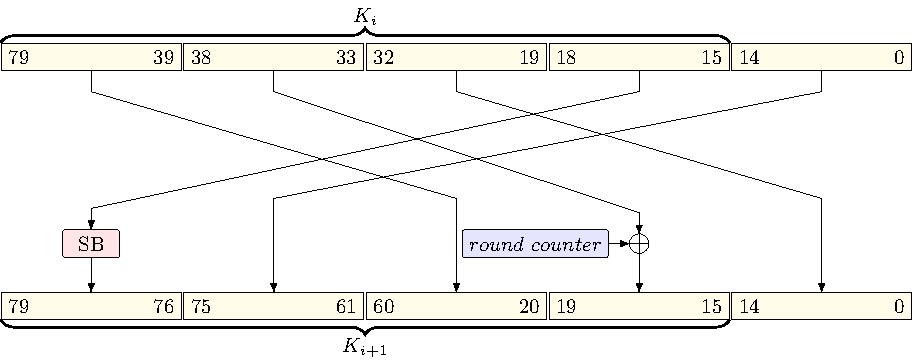
\includegraphics[width=0.8\textwidth]{fig/PRESENT_Key_Schedule.pdf}
\end{figure}
\begin{alertblock}{Remark}
    Knowledge of any round key for PRESENT-80 $\rightarrow64$ bits of the master key.
    The other $16$ bits can be recovered by brute force/knowledge of another round key
\end{alertblock}
\end{frame}